% !TeX root = ../sustechthesis-example.tex

\chapter[基于FPGA的RTMQ测控系统]{基于FPGA的RTMQ测控系统}

% \textcolor{red}{
% 这部分参考RTMQ的相关专利和文档介绍整个测控系统的情况... 
% }

量子物理实验系统常常涉及到一些物理量的精确调控和测量,这既包括量上的精确性,也包括时间上的精确性。因此量子物理实验系统对测量和控制性能提出了很多新的要求,其中十分关键的一点就是对测控系统实时性的要求。

目前实时系统在医疗、加工、汽车等行业都有较多的应用,实时系统具有响应快、延迟短等特点,其响应延迟和计时精度通常在毫秒至微秒量级,这一精度已经能满足当前诸多传统行业的控制需求。现有的实时系统一般使用主频在数百MHz至GHz量级的通用微处理器或微控制器作为控制的主体,以计时器中断和时间片分配等方式实现实时控制。这一方案成立的前提在于,所需的时间控制精度与指令执行频率之间有3-6个数量级的差异,因而通用处理器架构中存在的一些诸如分支预判、乱序执行等导致指令执行顺序不确定的因素以及中断系统中存在的现场保护、控制权交接等额外开销导致的时间控制不确定性可以忽略不计。

然而近来随着量子技术的发展,量子物理实验系统也开始产生对数据处理、复杂流程控制和实时控制的需求。不同于传统行业,量子物理实验系统对时间控制的精度和分辨率的要求在纳秒量级、延迟要求在百纳秒至数十微秒量级,与当前微处理器的主频相当,从而前述的现有的实时控制方案难以满足需求。

因此早年在量子物理实验领域内,通常用FPGA(现场可编程门阵列)设计特定的时序脉冲发生器来产生高时间精度的脉冲序列,以此作为其它实验设备的触发信号,进行准确的时序控制。然而,这种方案的灵活性较差,只能产生预定的序列,无法在实验中对实验数据进行即时的处理,或根据实验的中间结果对后续的流程进行及时的调整。近年来随着量子算法的发展,实验方案越来越复杂,实验流程中开始包含快速反馈的结构,即在实验过程中对实验目标进行测量,获得一些中间结果,而后对中间结果进行计算和处理,并进而确定后续的实验流程。中间结果的处理和后续流程的确定,一般要求在数十纳秒至数十微秒量级的时间内完成,并且执行时刻必须要严格确定。这要求实验的测控系统具有通用计算的能力,简单的时序脉冲发生器无法满足这一要求。

当前领域内针对此问题的主要解决思路为,另置一与时序脉冲发生器紧密连接的通用微处理器,用来对实验数据进行即时处理和产生时序脉冲发生器的后续输出时序。这一方案能较好的满足系统规模较小且实验时序不太复杂的情形下的实时控制需求。然而,这一方案的问题之一在于,微处理器和时序脉冲发生器依然是相互独立的两个个体,而微处理器的执行时序有其内在不确定性;二者之间要保持同步,或者需要频繁地相互交换触发信号,或者需要在时序设计上预留出充足的余量以覆盖此不确定性的最坏情形,总之都会复杂化时序的设计并产生时间浪费。

这一方案的另一问题在于,当系统规模较大,一个时序脉冲发生器无法控制整个系统时,就需要同时使用多个时序脉冲发生器,而一个微处理器同时处理过多的实验数据、同时控制过多的时序脉冲发生器,将不可避免的产生拥塞,这会进一步加剧前述的同步性问题。而如果同时使用多个微处理器,则不同微处理器之间的同步性又将成为问题;当前主流的微处理器架构和指令集都是针对通用计算而优化的,主流的微处理器使用的通信协议都是针对高吞吐率而优化的,二者都难以实现精确的时序同步。

\section[RTMQ实时系统架构介绍]{RTMQ实时系统架构介绍}

对于离子阱量子计算研究来说,一种实时性更强、拓展性更好、更灵活的测控系统十分重要。我们实验中对系统的控制和测量采用一种叫RTMQ的系统架构来实现。RTMQ系统架构提供了一种新的量子物理实验平台实时测控系统架构,解决了上述的不足。在RTMQ系统架构中,通用计算和时序控制由同一微处理器实现,因此避免了两个独立的模块之间同步性的问题;同时树状结构的系统中每个节点都具有通用计算的能力,因此可以实现计算任务的分布式处理,避免了拥塞的问题。

\begin{figure}
    \centering
    \caption[RTMQ系统架构示意图]{RTMQ系统架构示意图\label{fig:rtmq_nodes_and_leaves_structure}}
    \includegraphics[width=0.6\linewidth]{rtmq/rtmq_nodes_and_leaves_structure}
\end{figure}

RTMQ(用于量子物理实验的实时微系统,RealTime Microsystem for Quantum physics)架构主要用于基于FPGA或ASIC的兼具通用计算和高精度时序控制能力的微系统。系统的整体结构为树状结构,如图\ref{fig:rtmq_nodes_and_leaves_structure}所示,系统包含一个根节点,多个中间结点和多个叶节点;根节点通过网络、USB等方式与控制计算机相连。不同节点可位于同一PCB上,亦可位于不同PCB上。

\begin{figure}
    \centering
    \caption[RTMQ系统架构节点示意图]{RTMQ系统架构节点示意图\label{fig:rtmq_board_overal_structure}}
    \includegraphics[width=0.4\linewidth]{rtmq/rtmq_board_overal_structure}
\end{figure}

一般而言一个板卡具有如图\ref{fig:rtmq_board_overal_structure}所示的结构,板卡上的FPGA或ASIC包含一个RTMQ节点,RTMQ节点通过控制FPGA或ASIC的输入输出与数模/模数转换等各类功能芯片进行交互以实现所需功能,同时通过实时通信链路与其上级和下级节点连接。

\begin{figure}
    \centering
    \caption[RTMQ系统架构节点内部模块示意图]{RTMQ系统架构节点内部模块示意图\label{fig:rtmq_board_inner_structure}}
    \includegraphics[width=1.0\linewidth]{rtmq/rtmq_board_inner_structure}
\end{figure}

一个RTMQ节点的内部模块儿如图\ref{fig:rtmq_board_inner_structure}所示,包含一个32位的微处理器、一个寄存器文件、一系列外设模块和一个链路管理模块。其中微处理器包含流控制器、计时器、异常管理模块、触发管理模块和算术逻辑单元5个子模块;寄存器文件包含多个寄存器;外设可分为系统外设和功能外设,系统外设包括指令缓存、数据缓存、节点信息只读存储器以及地址栈和数据栈,功能外设用于实现具体的逻辑或时序功能,可包含多个。

RTMQ架构中包含的微处理器可受指令控制进入挂起状态,而挂起状态可受计时器或触发管理模块的控制恢复正常运行,如此,微处理器的指令流便可以按一定的时间间隔对齐或与外部信号对齐。同时,节点中的系统外设和功能外设的行为受关联寄存器的读写控制,即微处理器的指令与系统各模块的功能和时序有严格的对应关系。因此,本发明提供的架构可实现实时控制与通用计算在指令流层面的结合。
而配置指令插入中断的机制确保了节点对其下级节点的绝对控制,即使下级节点的微处理器处于挂起状态,依然不受影响。配置指令插入中断配合具有确定通信延迟的实时通信链路系统,即可实现时序确定的跨节点的即时反馈控制。

此外,RTMQ架构中每个节点都具有通用计算和时序控制能力,如此,大多数通用计算和时序生成都可以在叶节点或较近的中间结点完成,对于大规模系统不存在拥塞的问题,具有良好的可扩展性。


\section[测控硬件组成]{测控硬件组成}
\textcolor{red}{
1. 展示实物板卡照片;}

\begin{figure}
    \centering
    \caption[RTMQ测控板实物图]{RTMQ测控板实物图}
    \includegraphics[width=1.0\linewidth]{rtmq/rtmq_board_real}
\end{figure}

\textcolor{red}{
2. 结合照片给出主要器件清单及其介绍(参考专利:一种量子物理实验平台的实时测控系统架构);}



\section[软件API]{软件API}
\textcolor{red}{
1. 介绍软件API的功能和使用(可选,根据情况看吧,怎么介绍还没想好);}


\section[基于FPGA的数字超前进位加法器]{基于FPGA的数字超前进位加法器}
% \textcolor{red}{
% 1. 介绍数字加法器功能、逻辑图、Vivado中的实现、局限性;}

\subsection[加法器]{加法器}


加法器是一种用于执行加法运算的装置,在数字系统中有着广泛的用途。以下是几种常见的加法器结构:
\begin{itemize}
    \item 串行进位加法器(Carry Ripple Adder,CRA):这是最简单、最基本的加法器结构;
    \item 进位跳跃加法器(Carry Skip Adder,CKA);
    \item 进位选择加法器(Carry Select Adder,CSA);
    \item 超前进位加法器(Carry Lookahead Adder,CLA);
    \item 并行前缀加法器(Parallel Prefix Adder,PPA);
\end{itemize}
 
不同的加法器结构具有不同的性能和特点,在实际应用中,需要根据具体需求选择合适的加法器结构。

\subsection[超前进位加法器]{超前进位加法器}

加法器是构成运算器的基本部件,是构成乘法器、滤波器、数字PID等的基础和重要组成部分。量子测控系统要求高速的运算以实现对量子比特的精准调控,为提高运算速度,加法器一般都采用超前进位或先行进位方式。下面我将以超前进位加法器为例,介绍它的原理和在FPGA中的实现。

超前进位加法器指电路进行二进制加法运算时,通过快速进位电路同时产生除最低位全加器外的其余所有全加器的进位信号,无需再由低位到高位逐位传递进位信号,从而消除了串行进位加法器逐位传递进位信号的时间,提高了加法器的运算速度。

简单来说就是先用初始数据将各个进位都算出来,然后在经过一级全加器得出各个位的数据结果。

对于一个全加器,它的真值表如表\ref{tb:carry_ripple_adder}。其中$i_c$表示输入来自前一位的进位,$i_a, i_b$表示输入当前位待相加的两个数,$o_d$表示加法器输出结果的数据位;$o_c$表示加法器输出的向下一位的进位。
\begin{table}
    \centering
    \caption[串行进位加法器真值表]{串行进位加法器真值表。$i_c$表示输入来自前一位的进位;$i_a, i_b$表示输入当前位待相加的两个数;$o_d$表示加法器输出结果的数据位;$o_c$表示加法器输出的向下一位的进位。\label{tb:carry_ripple_adder}}
    \begin{tabular}{C{1.5cm}C{1.5cm}C{1.5cm}|C{1.5cm}C{1.5cm}}
        \toprule 
        \multicolumn{3}{c}{\textbf{Input}} & \multicolumn{2}{c}{\textbf{Output}}\\
        \toprule
        $i_c$ & $i_a$ & $i_b$ & $o_d$ & $o_c$\\
        \hline
        0 & 0 & 0 & 0 & 0 \\
        1 & 0 & 0 & 1 & 0 \\
        0 & 0 & 1 & 1 & 0 \\
        1 & 0 & 1 & 0 & 1 \\
        0 & 1 & 0 & 1 & 0 \\
        1 & 1 & 0 & 0 & 1 \\
        0 & 1 & 1 & 0 & 1 \\
        1 & 1 & 1 & 1 & 1 \\
        \bottomrule
    \end{tabular}
\end{table}

上述串行加法器的布尔表达式为:
\begin{align}
    o_d=&i_c \oplus i_a \oplus i_b\\
    Case1:
    o_c=&(i_a \cdot i_b) + (i_a \cdot i_c) + (i_b \cdot i_c)\\
    Case2:
    o_c=&i_c \cdot (i_a \oplus i_b) + i_a \cdot i_b\\
    Case3:
    o_c =& i_c \cdot (i_a + i_b) + i_a \cdot i_b
\end{align}

其中“$\oplus$”表示“异或”运算,“$\cdot$”表示“与”运算,“$+$”表示“或”运算。

\begin{figure}
    \centering
    \caption[串行进位加法器的FPGA实现结构图]{串行进位加法器的FPGA实现结构图\label{fig:carry_ripple_adder}(Vivado)}
    \includegraphics[width=1.0\linewidth]{rtmq/adder_case1}
    \includegraphics[width=1.0\linewidth]{rtmq/adder_case2}
    \includegraphics[width=1.0\linewidth]{rtmq/adder_case3}
\end{figure}

三种串行进位加法器实现的结构图如图\ref{fig:carry_ripple_adder}所示。从结果可以看到,第一种写法用了7个元件,输入到输出需要三级门电路得到结果;第二种写法用了5个器件,输入到输出需要三级门电路得到结果;第三种写法用了6个元件,输入到输出需要三级门电路得到结果;从器件数量角度优选地应该使用第二种写法,具体还取决于系统可用的元器件情况。可以看出当前位对下一位的数据和进位逻辑如下:

\begin{align}
    d_i =& a_i\oplus b_i \oplus c_i\\
    c_{i+1}=& a_i \cdot b_i +(a_i \oplus b_i)\cdot c_i = G_i + (P_i)\cdot c_i
\end{align}

其中$G_i=a_i \cdot b_i$是生成信号,$P_i=a_i \oplus b_i$是传播信号。如果想要消除进位依赖,那么进位$c_{i+1}$的表达式就不能有$c_i, c_{i-1}, \dots, c_i$项,$c_0$项为初始赋予不需要替换。这里考虑四位超前进位加法器设计如下:

\begin{align}
    c_0 &= c_0\\
    c_1 &= G_0 + P_0 c_0\\
    c_2 &= G_1 + P_1 c_1 = G_1+P_1 (G_0+P_0 c_0 )=G_1+P_1 G_0+P_1 P_0 c_0\\
    c_3 &=G_2+P_2 c_2=G_2+P_2 (G_1+P_1 G_0+P_1 P_0 c_0 )\\
    &=G_3+P_3 G_2+P_3 P_2 G_1+P_3 P_2 P_1 P_0 c_0\\
    c_5 &=G_4+P_4 c_4=G_4+P_4 (G_3+P_3 G_2+P_3 P_2 G_1+P_3 P_2 P_1 P_0 c_0 )\\
    \dots\\
    c_{i+1} &=G_i+P_i G_{i-1}+P_i P_{i-1} G_{i-2}+ \dots +\prod_0^i P_j \cdot c_0
\end{align}

从中可见,对于第$i+1$位进位的计算$P_i$要参加$i+1$组计算。超前进位加法器的FPGA实现结构图如图\ref{fig:ahead_adder_4bits}所示。

\begin{figure}
    \centering
    \caption[4位超前进位加法器的FPGA实现结构图]{4位超前进位加法器的FPGA实现结构图(Vivado)\label{fig:ahead_adder_4bits}}
    \includegraphics[width=1.0\linewidth]{rtmq/ahead_adder_4bits}
\end{figure}

按照上述规律进行拓展,可以依次得到需求位数的超前进位加法器,比如8位(图\ref{fig:ahead_adder_8bits})、16位(图\ref{fig:ahead_adder_16bits})、32位(图\ref{fig:ahead_adder_32bits})等。值得注意的是,理论上使用超前进位方式可以实现任意位数的加法器,并且实现的加法器只需要两级流水线就可以得到最终结果。不过实际上高速数字电路的延时不仅有流水线延时,还有器件延时。可以看到超前进位加法器从4位(图\ref{fig:ahead_adder_4bits})到32位(图\ref{fig:ahead_adder_32bits}),在超前进位计算的逻辑有了相当程度的复杂化了。受到器件压时延的限制,我们无法超前计算无限位数的超前进位$c_{\infty}$。
\begin{figure}
    \centering
    \caption[8位超前进位加法器的FPGA实现结构图]{8位超前进位加法器的FPGA实现结构图(Vivado)\label{fig:ahead_adder_8bits}}
    \includegraphics[width=1.0\linewidth]{rtmq/ahead_adder_8bits}
\end{figure}

\begin{figure}
    \centering
    \caption[16位超前进位加法器的FPGA实现结构图]{16位超前进位加法器的FPGA实现结构图(Vivado)\label{fig:ahead_adder_16bits}}
    \includegraphics[width=1.0\linewidth]{rtmq/ahead_adder_16bits}
\end{figure}

\begin{figure}
    \centering
    \caption[32位超前进位加法器的FPGA实现结构图]{32位超前进位加法器的FPGA实现结构图(Vivado)\label{fig:ahead_adder_32bits}}
    \includegraphics[width=1.0\linewidth]{rtmq/ahead_adder_32bits}
\end{figure}
\begin{figure}
    \centering
    \caption[用两个32位超前进位加法器拓展为一个64位加法器]{用两个32位超前进位加法器拓展为一个64位加法器(Vivado)\label{fig:adder_64bits}}
    \includegraphics[width=1.0\linewidth]{rtmq/adder_64bits}
\end{figure}

一般情况下32位加法器就足够用了,比如RTMQ系统就是采用32位运算的。如果需要更高位数的加法器可以继续向上拓展,也可以考虑用串行进位加法器的思想对超前进位加法器进行拓展。

如图\ref{fig:adder_64bits}所示,这里用了两个32位加法器添加了一级流水线,拓展为了一个64位的加法器。用这种方式可以满足一些特殊的更高位数加法器的实现。不过,在流水线时延上要做出一点妥协。







\newpage
\section[基于FPGA的数字Booth乘法器]{基于FPGA的数字Booth乘法器}
% \textcolor{red}{
% 1. 介绍数字Booth乘法器功能、逻辑图、Vivado中的实现、优势;}
布斯(Booth)乘法器是一种对乘数进行重新编码,以减少乘法运算中所需的加法次数的乘法器。它由布斯夫妇于 1950 年发明,因硬件实现简单、所需硅片面积较小、能够显著提高乘法运算速度而被广泛采用。

Booth乘法器通过相加和相减的操作计算补码数据的乘积。该算法对乘数从低位开始判断,根据后两个数据位的情况决定进行加法、减法还是仅仅进行移位操作。
在计算两个补码相乘时,会将上一轮编码产生的进位与当前轮编码进行相加,然后再进行移位操作。通过这种方式,布斯乘法器可以减少乘法运算中所需的加法次数,从而提高计算速度。

Booth乘法器在数字信号处理、计算机算术、密码学等领域中具有广泛的应用。在RTMQ系统中有关的乘法运算基本都是以Booth乘法器来实现的。下面将介绍它的原理和实现。

进位保留加法器编码(3to2编码)如图\ref{fig:carray_save_adder_clock}所示。
\begin{figure}
    \centering
    \caption[进位保留加法器编码(3to2编码)]{进位保留加法器编码(3to2编码)\label{fig:carray_save_adder_clock}}
    \includegraphics[width=1.0\linewidth]{rtmq/carray_save_adder_clock}
\end{figure}


8位Booth乘法器的编码表和编程设计图如图\ref{fig:booth_multiplier_8bits_basic}所示。
\begin{figure}
    \centering
    \caption[16位Booth乘法器编码表]{16位Booth乘法器编码表\label{fig:booth_multiplier_8bits_basic}}
    \includegraphics[width=1.0\linewidth]{rtmq/booth_multiplier_8bits_basic}
\end{figure}



16位Booth乘法器的编程设计图如图\ref{fig:booth_multiplier_16bits_basic}所示。相应的结构示意图如图所示。
\begin{figure}
    \centering
    \caption[16位Booth乘法器编码表]{16位Booth乘法器编码表\label{fig:booth_multiplier_16bits_basic}}
    \includegraphics[width=1.0\linewidth]{rtmq/booth_multiplier_16bits_basic}
\end{figure}

\begin{figure}
    \centering
    \caption[16位Booth乘法器结构示意图]{16位Booth乘法器结构示意图\label{fig:booth_multiplier_16bits_basic_s}}
    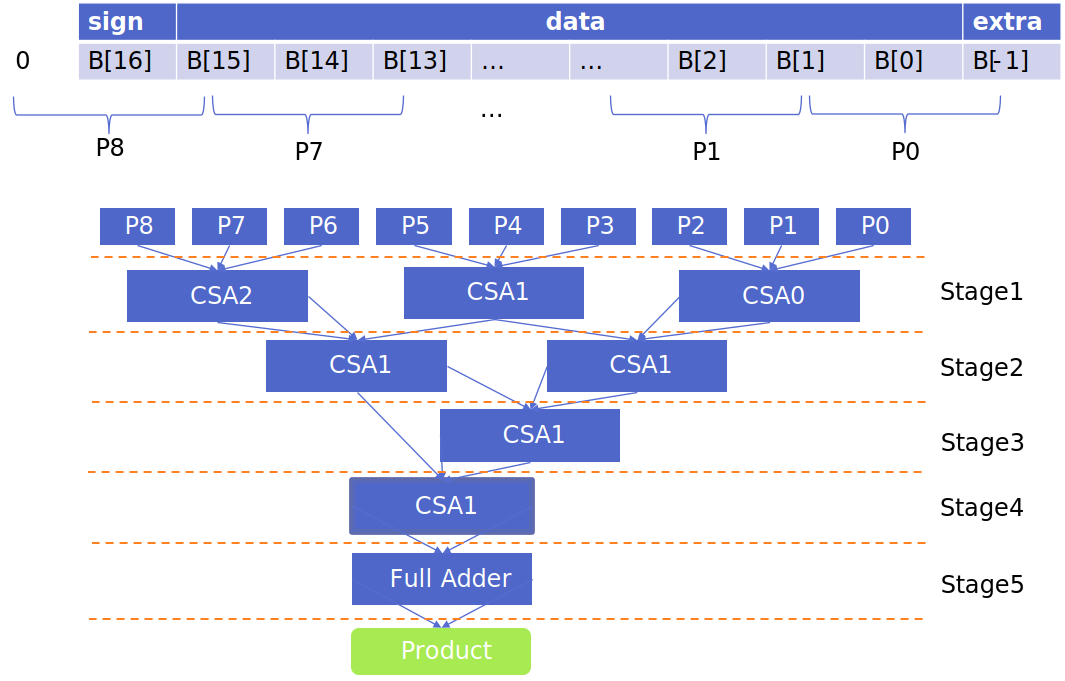
\includegraphics[width=1.0\linewidth]{rtmq/booth_multiplier_16bits_basic_s}
\end{figure}


更高位数的Booth乘法器实现可以依据上述规律进行设计开发。


\newpage
\section[基于FPGA的数字PID]{基于FPGA的数字PID}
% \textcolor{red}{
% 1. 介绍数字PID功能、逻辑图、Vivado中的实现、优势;}

16位数字滤波器结构示意图如图\ref{fig:digital_pid_structure_16bits_s}所示。相应的FPGA实现结构图如图\ref{fig:digital_pid_structure_16bits}所示。
\begin{figure}
    \centering
    \caption[16位数字滤波器结构示意图]{16位数字滤波器结构示意图\label{fig:digital_pid_structure_16bits_s}}
    \includegraphics[width=1.0\linewidth]{rtmq/digital_pid_structure_16bits_s}
\end{figure}

\begin{figure}
    \centering
    \caption[16位数字滤波器FPGA实现结构图]{16位数字滤波器FPGA实现结构图\label{fig:digital_pid_structure_16bits}}
    \includegraphics[width=1.0\linewidth]{rtmq/digital_pid_structure_16bits}
\end{figure}






\section[基于FPGA的通用数字滤波器]{基于FPGA的通用数字滤波器}
\textcolor{red}{
1. 介绍数字滤波器功能、种类、基本原理,比如有限冲激响应滤波器、无限冲激响应滤波器等等;}

\textcolor{red}{
2. 介绍数字通用滤波器功能、逻辑图、Vivado中的实现、优势;}




